\section{Consuntivo di periodo}
Di seguito verranno indicate le spese effettivamente sostenute da ogni ruolo. Il bilancio di consuntivo potrà risultare: \begin{itemize}
\item \textbf{Positivo}: se il preventivo supera il consuntivo;
\item \textbf{Pari}: se preventivo e consuntivo sono uguali;
\item \textbf{Negativo}: se il consuntivo supera il preventivo.
\end{itemize}

\subsection{Periodo di Analisi}
%tabella costi
\begin{table}[H]
\centering\renewcommand{\arraystretch}{1.5}
\caption{Consuntivo del periodo di Analisi}
\vspace{0.2cm}
\begin{tabular}{ c c c }
\rowcolor{redafk}
\textcolor{white}{\textbf{Ruolo}} & \textcolor{white}{\textbf{Ore}} & 
\textcolor{white}{\textbf{Costo}}  \\
Responsabile & 34 & 1020€ \\
Amministratore & 41 (+13) & 820€ (+260€) \\
Analista & 107 (+8) & 2675€ (+200€) \\
Progettista	& 24 & 528€  \\
Programmatore & 0 & 0€  \\
Verificatore & 82 (+9) & 1230€ (+135€)  \\
\textbf{Totale preventivo} & \textbf{288} & \textbf{6273€}  \\
\textbf{Totale consuntivo} & \textbf{318} & \textbf{6868€}  \\
\rowcolor{lastrowcolor}
\textbf{Differenza} & \textbf{+30} & \textbf{+595€}  \\
\end{tabular}
\end{table}

\subsubsection{Conclusioni}
Come emerge dai dati riportati nella tabella soprastante è stato necessario investire più tempo del previsto nei ruoli di \textit{Amministratore}, \textit{Analista} e \textit{Verificatore}. Per questo motivo il bilancio risultante è negativo. Le cause di tali ritardi sono riportate di seguito:
\begin{itemize}
\item \textbf{\textit{Amministratore}}: è servito più tempo del previsto per riuscire ad individuare i software più adatti per la gestione del progetto e per la loro  configurazione. Inoltre sono state aggiunte ed aggiornate alcune sezioni nelle \textit{Norme di Progetto}, necessarie al chiarimento di alcune problematiche sorte durante la stesura dei documenti;
\item \textbf{\textit{Analista}}: alcuni requisiti si sono rivelati di non facile comprensione, e sono state necessarie più ore di lavoro per la discussione interna tra gli \textit{Analisti} ed esterna con il proponente;
\item \textbf{\textit{Verificatore}}: l’aggiunta di nuove sezioni nelle \textit{Norme di Progetto} e l'inesperienza dei membri hanno implicato un maggiore lavoro anche per questo ruolo.
\end{itemize}
Il notevole quantitativo di ore che il gruppo ha dovuto impiegare nel primo periodo non deve ripetersi durante il lavoro rendicontato. Per le problematiche riscontrate verranno adottate le seguenti contromisure:
\begin{itemize}
	\item amministrazione degli strumenti: il gruppo ha ricercato e configurato in anticipo gli strumenti che verranno usati. In caso venissero individuati nuovi strumenti avere già un ambiente di sviluppo impostato correttamente per tutti i membri semplificherà la nuova configurazione e ridurrà l'insorgere di problemi;
	\item comprensione dei requisiti: i requisiti sono stati ampiamente discussi con il proponente durante questa fase, non si prevede di incorrere ulteriormente in tale problema;
	\item applicazione delle norme: i membri del gruppo hanno studiato attentamente le norme, in modo tale da poter redigere fin da subito nuove sezioni dei documenti già normate, semplificando il lavoro ai verificatori.
\end{itemize}

\subsubsection{Preventivo a finire}
Essendo questo periodo non rendicontato, non vengono a generarsi problemi nel monte ore totale, nonché nel preventivo economico. Nonostante ciò \textit{TeamAFK} si impegnerà a integrare altre misure di contenimento ad eventuali nuovi problemi, facendo esperienza dei problemi riscontrati durante questo primo periodo

\subsection{Periodo di Progettazione e codifica per la Technology Baseline}

\begin{table}[H]
\centering\renewcommand{\arraystretch}{1.5}
\caption{Consuntivo del periodo di Progettazione e codifica per la Technology Baseline}
\vspace{0.2cm}
\begin{tabular}{ c c c }
\rowcolor{redafk}
\textcolor{white}{\textbf{Ruolo}} & \textcolor{white}{\textbf{Ore}} &
\textcolor{white}{\textbf{Costo}}  \\
Responsabile 	& 12 & 360€ \\
Amministratore 	& 20 (+9) 	& 400€ (+180€) \\
Analista 		& 35 (-20) 	& 875€ (-500€) \\
Progettista		& 59 (+8) 	& 1298€ (+176€)\\
Programmatore	& 33 (+13) 	& 495€ (+195€)\\
Verificatore 	& 53 & 795€ \\
\textbf{Totale preventivo} & \textbf{212} & \textbf{4223€}  \\
\textbf{Totale consuntivo} & \textbf{222} & \textbf{4274€}  \\
\rowcolor{lastrowcolor}
\textbf{Differenza} & \textbf{+10} & \textbf{+51€}  \\
\end{tabular}
\end{table}

\subsubsection{Analisi degli incrementi}
Al fine di garantire uno sviluppo del progetto congruo con quanto preventivato
nei tempi e nei costi, gli incrementi individuati nella pianificazione sono stati sviluppati in parallelo. Terminata la fase di codifica, si rilevano eventuali problemi riscontrati ed eventualmente si modifica e si dettaglia ulteriormente la pianificazione futura in modo da mitigare gli effetti di questi imprevisti.

\paragraph*{Incremento 1} \mbox{} \\ \mbox{} \\
Il tempo dedicato alla codifica di questo incremento e le risorse assegnategli sono risultati ben bilanciati. I programmatori dedicati sono riusciti a sviluppare quanto pianificato entro la scadenza prefissata. \\ 
Terminato il proprio compito, quest'ultimi si sono messi a disposizione dei propri colleghi.

\paragraph*{Incremento 2} \mbox{} \\ \mbox{} \\
La codifica di questo incremento ha avuto dei rallentamenti dovuti all'inesperienza dei programmatori con tale tecnologia unita alla scarsa documentazione fornita da Grafana. \\ Il \textit{TeamAFK} ha sfruttato questo periodo per incrementare le proprie conoscenze ed abilità in relazione all'ambiente di sviluppo e ai linguaggi di programmazione necessari allo sviluppo di tale e future funzionalità. 

\paragraph*{Incremento 3} \mbox{} \\ \mbox{} \\
La codifica di questo incremento, come per l'incremento 2, ha avuto dei rallentamenti dovuti all'inesperienza dei programmatori con tale tecnologia unita alla scarsa documentazione fornita da Grafana. \\ 
Il \textit{TeamAFK} ha pertanto sfruttato questo periodo per incrementare le proprie conoscenze ed abilità in relazione all'ambiente di sviluppo e ai linguaggi di programmazione necessari allo sviluppo di tale e future funzionalità.

\subsubsection{Conclusioni}
Come emerge dai dati riportati nella tabella soprastante è stato necessario investire più tempo nei ruoli di \textit{Amministratore}, \textit{Progettista} e \textit{Programmatore} mentre l'\textit{Analista} ha visto una riduzione delle sue ore. Le cause di tali scostamenti sono riportate di seguito:
\begin{itemize}
	\item \textbf{\textit{Amministratore}}: la causa di questo aumento di ore è dovuto all'aggiunta e modifica di alcune parti delle \textit{Norme di Progetto};
	\item \textbf{\textit{Analista}}: l'elevata comunicazione con il proponente nel periodo di analisi ha permesso un'ottima comprensione del prodotto da sviluppare, questo ha permesso di concentrarsi principalmente sulla correzione dell'\textit{Analisi dei Requisiti};
	\item \textbf{\textit{Progettista}}: le ore aggiuntive sono state richieste per la correzione del documento \textit{Priano di Qualifica};
	\item \textbf{\textit{Programmatore}}: data l'inesperienza con le tecnologie utilizzate per lo sviluppo del software, sono state richieste più ore di programmazione per comprendere e quindi correggere i problemi che si sono presentati durante la codifica delle funzionalità previste per la PoC.
\end{itemize}

Rispetto alla fase di analisi, le ore aggiunte sono decisamente ridotte, però in questo caso le ore sono rendicontate, quindi lo sforamento è ben più grave. Per le problematiche riscontrate verranno adottate le seguenti contromisure: 
\begin{itemize}
	\item mancanza ed errata stesura di alcune sezioni delle norme: è stata prestata particolare attenzione durante la correzione, in modo tale che non si debbano correggere ulteriormente le \textit{Norme di Progetto} in futuro;
	\item correzione dei documenti: durante la stesura e la verifica si è stati più meticolosi, così da ridurre il più possibile eventuali nuove correzioni;
	\item inesperienza tecnologica: durante questa fase si è analizzato le componenti del prodotto che potrebbero essere più complicate, ricercando in anticipo informazioni ed possibili soluzioni.
\end{itemize}

\subsubsection{Preventivo a finire}
Il bilancio risultante è negativo, in quanto sono stati spesi 51€ in più rispetto a quanto preventivato. Per questo motivo sarà necessario impegnarsi per ridurre il costo dei successivi periodi senza però intaccare la qualità del prodotto finale.

\subsection{Periodo di progettazione di dettaglio e codifica}
\label{tab:pb}
\begin{table}[H]
\centering\renewcommand{\arraystretch}{1.5}
\caption{Consuntivo del periodo di progettazione di dettaglio e codifica}
\vspace{0.2cm}
\begin{tabular}{ c c c }
\rowcolor{redafk}
\textcolor{white}{\textbf{Ruolo}} & \textcolor{white}{\textbf{Ore}} &
\textcolor{white}{\textbf{Costo}}  \\
Responsabile 	& 18 & 540€ \\
Amministratore 	&  23	& 460€ \\
Analista 		& 0 (+6)  & 0 (+150€) \\
Progettista		&  74 (-8) & 1628€ (-176€)\\
Programmatore	&  	140 (-4)& 2100€ (-60€)\\
Verificatore 	& 83 (+2) &  1245€ (+30€)\\
\textbf{Totale preventivo} & \textbf{338} & \textbf{5973€}  \\
\textbf{Totale consuntivo} & \textbf{334} & \textbf{5917€} \\
\rowcolor{lastrowcolor}
\textbf{Differenza} & \textbf{-4} & \textbf{-56€} \\
\end{tabular}
\end{table}

\subsubsection{Analisi degli incrementi}
Di seguito sono analizzati tutti gli incrementi singolarmente, ed ognuno contiene una breve descrizione dei costi, negativi o positivi, presenti nella tabella.

\paragraph*{Incremento 4} \mbox{} \\ \mbox{} \\
Come riportato nella tabella seguente, la codifica di questo incremento ha richiesto meno tempo di quello preventivato, in quanto i \textit{Programmatori} avevano acquisito le conoscenze necessarie allo sviluppo di quest'ultimo nella fase precedente di Progettazione e codifica per la Technology Baseline (in particolare durante lo sviluppo dell'incremento 1). Sono state apportate inoltre delle piccole modifiche alla struttura del codice.
\begin{table}[H]
\centering\renewcommand{\arraystretch}{1.5}
\caption{Consuntivo dell'incremento 4}
\vspace{0.2cm}
\begin{tabular}{ c c c }
\rowcolor{redafk}
\textcolor{white}{\textbf{Ruolo}} & \textcolor{white}{\textbf{Ore}} &
\textcolor{white}{\textbf{Costo}}  \\
Responsabile 	& 2 & 60€ \\
Amministratore 	&  4 & 80€ \\
Analista 		&  0 & 0€ \\
Progettista		&  4 (-1) & 88€ (-22€)\\
Programmatore	&  14 (-2) & 240€ (-30€)\\
Verificatore 	& 6 & 90€ \\
\textbf{Totale preventivo} & \textbf{32} & \textbf{558€}  \\
\textbf{Totale consuntivo} & \textbf{29} & \textbf{506€}  \\
\rowcolor{lastrowcolor}
\textbf{Differenza} & \textbf{-3} & \textbf{-52€} \\
\end{tabular}
\end{table}

\paragraph*{Incremento 5} \mbox{} \\ \mbox{} \\
Come riportato nella tabella seguente, la codifica di questo incremento ha rispettato le tempistiche e i costi preventivati.
\begin{table}[H]
\centering\renewcommand{\arraystretch}{1.5}
\caption{Consuntivo dell'incremento 5}
\vspace{0.2cm}
\begin{tabular}{ c c c }
\rowcolor{redafk}
\textcolor{white}{\textbf{Ruolo}} & \textcolor{white}{\textbf{Ore}} &
\textcolor{white}{\textbf{Costo}}  \\
Responsabile 	& 1 & 30€ \\
Amministratore 	& 1 & 20€ \\
Analista 		& 0 & 0€ \\
Progettista		& 1 & 22€ \\
Programmatore	& 3 & 45€ \\
Verificatore 	& 2 & 30€ \\
\textbf{Totale preventivo} & \textbf{8} & \textbf{147€}  \\
\textbf{Totale consuntivo} & \textbf{8} & \textbf{147€}  \\
\rowcolor{lastrowcolor}
\textbf{Differenza} & \textbf{0} & \textbf{0€} \\
\end{tabular}
\end{table}

\paragraph*{Incremento 6} \mbox{} \\ \mbox{} \\
Come riportato nella tabella seguente, la codifica di questo incremento ha subito una leggera variazione, positiva, in quanto è stato implementato quanto necessario leggermente più velocemente rispetto a quanto pianificato.
\begin{table}[H]
\centering\renewcommand{\arraystretch}{1.5}
\caption{Consuntivo dell'incremento 6}
\vspace{0.2cm}
\begin{tabular}{ c c c }
\rowcolor{redafk}
\textcolor{white}{\textbf{Ruolo}} & \textcolor{white}{\textbf{Ore}} &
\textcolor{white}{\textbf{Costo}}  \\
Responsabile 	& 3 & 90€ \\
Amministratore 	& 4 & 80€ \\
Analista 		& 0  & 0€ \\
Progettista		& 6  &  132€\\
Programmatore	& 14 & 225€ (-15€) \\
Verificatore 	& 6 & 90€ \\
\textbf{Totale preventivo} & \textbf{34} & \textbf{617€}   \\
\textbf{Totale consuntivo} & \textbf{33} & \textbf{602€}  \\
\rowcolor{lastrowcolor}
\textbf{Differenza} & \textbf{-1} & \textbf{-15€} \\
\end{tabular}
\end{table}

\paragraph*{Incremento 7} \mbox{} \\ \mbox{} \\
Come riportato nella tabella seguente, la codifica di questo incremento ha richiesto meno ore di progettazione, in quanto l'architettura necessaria al suo sviluppo è stata ben definita dai \textit{Progettisti} e i \textit{Programmatori} non hanno avuto necessità di chiedere maggiori informazioni.
\begin{table}[H]
\centering\renewcommand{\arraystretch}{1.5}
\caption{Consuntivo dell'incremento 7}
\vspace{0.2cm}
\begin{tabular}{ c c c }
\rowcolor{redafk}
\textcolor{white}{\textbf{Ruolo}} & \textcolor{white}{\textbf{Ore}} &
\textcolor{white}{\textbf{Costo}}  \\
Responsabile 	& 2 & 60€ \\
Amministratore 	& 2 &  40€ \\
Analista 		& 0  & 0€ \\
Progettista		& 10 (-2)  & 220€ (-44€) \\
Programmatore	&  6 & 90€ \\
Verificatore 	&  4 & 60€ \\
\textbf{Totale preventivo} & \textbf{24} & \textbf{470€}  \\
\textbf{Totale consuntivo} & \textbf{22} & \textbf{426€}  \\
\rowcolor{lastrowcolor}
\textbf{Differenza} & \textbf{-2} & \textbf{-44€} \\
\end{tabular}
\end{table}

\paragraph*{Incremento 8} \mbox{} \\ \mbox{} \\
Come riportato nella tabella seguente, la codifica di questo incremento ha richiesto piu soldi (e ore) di quanto preventivato, in quanto sono stati riscontrati dei problemi nell'\textit{Analisi dei Requisiti}, da risolvere subito e nel minor tempo possibile. Tal'ultimi hanno richiesto 6 ore di analisi in più di quanto preventivato inizialmente.\\
La progettazione, invece, ha richiesto 1 ora in meno per mettere a punto e sviluppare l'idea architetturale dietro a questo incremento.
\begin{table}[H]
\centering\renewcommand{\arraystretch}{1.5}
\caption{Consuntivo dell'incremento 8}
\vspace{0.2cm}
\begin{tabular}{ c c c }
\rowcolor{redafk}
\textcolor{white}{\textbf{Ruolo}} & \textcolor{white}{\textbf{Ore}} &
\textcolor{white}{\textbf{Costo}}  \\
Responsabile 	& 3 & 90€ \\
Amministratore 	& 4 & 80€ \\
Analista 		& 0 (+6)  & 0 (+150€) \\
Progettista		& 8 (-1)  & 176€ (-22€) \\
Programmatore	& 20 & 300€ \\
Verificatore 	& 11 & 165€  \\
\textbf{Totale preventivo} & \textbf{46} & \textbf{811€}  \\
\textbf{Totale consuntivo} & \textbf{51} & \textbf{939€} \\
\rowcolor{lastrowcolor}
\textbf{Differenza} & \textbf{+5} & \textbf{+128€} \\
\end{tabular}
\end{table}

\paragraph*{Incremento 9} \mbox{} \\ \mbox{} \\
Come riportato nella tabella seguente, la codifica di questo incremento ha richiesto meno ore di progettazione, in quanto la sua struttura era già ben definita. 
\begin{table}[H]
\centering\renewcommand{\arraystretch}{1.5}
\caption{Consuntivo dell'incremento 9}
\vspace{0.2cm}
\begin{tabular}{ c c c }
\rowcolor{redafk}
\textcolor{white}{\textbf{Ruolo}} & \textcolor{white}{\textbf{Ore}} &
\textcolor{white}{\textbf{Costo}}  \\
Responsabile 	& 2 & 60€ \\
Amministratore 	& 4 & 80€ \\
Analista 		&  0 & 0€ \\
Progettista		&  15 (-4) & 330€ (-88€) \\
Programmatore	&  27 (-1) & 405€ (-15€) \\
Verificatore 	&  20 & 300€ \\
\textbf{Totale preventivo} & \textbf{68} & \textbf{1175€}  \\
\textbf{Totale consuntivo} & \textbf{63} & \textbf{1072€}  \\
\rowcolor{lastrowcolor}
\textbf{Differenza} & \textbf{-5} & \textbf{-103€} \\
\end{tabular}
\end{table}

\paragraph*{Incremento 10} \mbox{} \\ \mbox{} \\
Come riportato nella tabella seguente, la codifica di questo incremento ha rispetto quanto preventivato.
\begin{table}[H]
\centering\renewcommand{\arraystretch}{1.5}
\caption{Consuntivo dell'incremento 1o}
\vspace{0.2cm}
\begin{tabular}{ c c c }
\rowcolor{redafk}
\textcolor{white}{\textbf{Ruolo}} & \textcolor{white}{\textbf{Ore}} &
\textcolor{white}{\textbf{Costo}}  \\
Responsabile 	& 1 & 30€ \\
Amministratore 	& 1 & 20€ \\
Analista 		& 0 & 0€ \\
Progettista		& 7 & 154€ \\
Programmatore	& 11 & 165€\\
Verificatore 	& 9 &  135€\\
\textbf{Totale preventivo} & \textbf{29} & \textbf{504€}  \\
\textbf{Totale consuntivo} & \textbf{29} & \textbf{504€}  \\
\rowcolor{lastrowcolor}
\textbf{Differenza} & \textbf{0} & \textbf{0€} \\
\end{tabular}
\end{table}

\paragraph*{Incremento 11} \mbox{} \\ \mbox{} \\
Come riportato nella tabella seguente, la codifica di questo incremento ha richiesto due ore in più di verifica in quanto lo sviluppo di alcuni test ha richiesto più tempo del previsto data l'inesperienza del \textit{TeamAFK} con questo tipologia di codifica.
\begin{table}[H]
\centering\renewcommand{\arraystretch}{1.5}
\caption{Consuntivo dell'incremento 11}
\vspace{0.2cm}
\begin{tabular}{ c c c }
\rowcolor{redafk}
\textcolor{white}{\textbf{Ruolo}} & \textcolor{white}{\textbf{Ore}} &
\textcolor{white}{\textbf{Costo}}  \\
Responsabile 	& 2 & 60€  \\
Amministratore 	& 3	& 60€\\
Analista 		& 0  & 0€ \\
Progettista		& 11 & 242€ \\
Programmatore	& 18 & 270€ \\
Verificatore 	& 12 (+2) & 150€ (+30€) \\
\textbf{Totale preventivo} & \textbf{44} & \textbf{782€}  \\
\textbf{Totale consuntivo} & \textbf{46} & \textbf{812€}  \\
\rowcolor{lastrowcolor}
\textbf{Differenza} & \textbf{+2} & \textbf{+30€} \\
\end{tabular}
\end{table}

\paragraph*{Incremento 12} \mbox{} \\ \mbox{} \\
Come riportato nella tabella seguente, la codifica di questo incremento ha rispetto quanto preventivato.
\begin{table}[H]
\centering\renewcommand{\arraystretch}{1.5}
\caption{Consuntivo dell'incremento 12}
\vspace{0.2cm}
\begin{tabular}{ c c c }
\rowcolor{redafk}
\textcolor{white}{\textbf{Ruolo}} & \textcolor{white}{\textbf{Ore}} &
\textcolor{white}{\textbf{Costo}}  \\
Responsabile 	& 2 & 60€ \\
Amministratore 	& 0 & 0€ \\
Analista 		&  0 & 0€ \\
Progettista		&  12 & 264€ \\
Programmatore	&  24 & 360€ \\
Verificatore 	&  15 & 225€ \\
\textbf{Totale preventivo} & \textbf{53} & \textbf{909€}  \\
\textbf{Totale consuntivo} & \textbf{53} & \textbf{909€}  \\
\rowcolor{lastrowcolor}
\textbf{Differenza} & \textbf{0} & \textbf{0€} \\
\end{tabular}
\end{table}


\subsubsection{Conclusioni generali}
Come emerge dai dati riportati nella tabella \hyperref[tab:pb]{6.3.1 }è stato necessario investire più tempo nei ruoli di \textit{Analista} e \textit{Verificatore} mentre il \textit{Programmatore} e il \textit{Progettista} hanno visto una riduzione delle loro ore. Le cause di tali scostamenti sono riportate di seguito:
\begin{itemize}
	\item \textbf{\textit{Analista}}: è stato necessario rivedere la struttura dei casi d'uso e l'importanza di alcuni requisiti, in modo da soddisfare e rispettare il \textit{Piano di Progetto}. Infine, sono state apportate le correzioni indicate dal committente;
	\item \textbf{\textit{Progettista}}: i \textit{Progettisti} avevano studiato, descritto e impostato in modo esaustivo l'architettura del prodotto nella fase precedente; è stato richiesto quindi meno tempo per progettare quanto codificato e mostrato durante la Product Baseline e la Revisione di Qualifica; 
	\item \textbf{\textit{Programmatore}}: sono state richieste meno ore di programmazione per sviluppare quanto descritto in questo documento, data l'esperienza acquisita durante la Technology Baseline;
	\item \textbf{\textit{Verificatore}}: sono state richieste più ore di verifica, in quanto sono stati riscontrati dei problemi nella stesura dei test; nessun membro del \textit{TeamAFK} aveva esperienza con questo tipo di codifica.
\end{itemize}
Rispetto alla fase di Progettazione e codifica per la Technology Baseline, le ore aggiunte sono dovute principalmente all'inesperienza del \textit{TeamAFK} nella stesura di codice di test. \\
Per le problematiche riscontrate verranno adottate le seguenti contromisure: 
\begin{itemize}
	\item correzione dei documenti: durante la stesura e la verifica si è stati più meticolosi, così da ridurre il più possibile eventuali nuove correzioni;
	\item inesperienza tecnologica: questo periodo ha permesso al \textit{TeamAFK} di sviluppare nuove conoscenze. Quest'ultime velocizzeranno il processo di codifica del periodo successivo, in cui il progetto dovrà essere terminato del tutto.
\end{itemize}


\subsubsection{Preventivo a finire generale}
Le modifiche apportate alla pianificazione ci hanno permesso di avere un
bilancio positivo. Tale bilancio risulta tale in quanto i costi che abbiamo effettivamente rilevato sono inferiori a quelli che erano stati preventivati (-56€). Questi soldi risparmiati vengono utilizzati per coprire le spese in eccesso del periodo precedente.\\
Per quanto riguarda lo sviluppo degli incrementi, il \textit{TeamAFK} si ritiene soddisfatto di quanto prodotto in questo periodo.


\subsection{Periodo di Validazione e collaudo}
\label{tab:pb}
\begin{table}[H]
\centering\renewcommand{\arraystretch}{1.5}
\caption{Consuntivo del periodo di validazione e collaudo}
\vspace{0.2cm}
\begin{tabular}{ c c c }
\rowcolor{redafk}
\textcolor{white}{\textbf{Ruolo}} & \textcolor{white}{\textbf{Ore}} &
\textcolor{white}{\textbf{Costo}}  \\
Responsabile 	& 20 & 600€ \\
Amministratore 	&  23 (-8)	& 460€ (-160€) \\
Analista 		& 0 (+3)  & 0€ (+75€)  \\
Progettista		& 12 (+5)  & 264€ (+110€) \\
Programmatore	& 25 (+14) & 375€ (+210€) \\
Verificatore 	& 93 (-16) &  1395€ (-240€) \\
\textbf{Totale preventivo} & \textbf{173} & \textbf{3094€} \\
\textbf{Totale consuntivo} & \textbf{171} & \textbf{3089€} \\
\rowcolor{lastrowcolor}
\textbf{Differenza} & \textbf{-2} & \textbf{-5€} \\
\end{tabular}
\end{table}

\subsubsection{Analisi degli incrementi}
Di seguito sono analizzati tutti gli incrementi singolarmente, ed ognuno contiene una breve descrizione dei costi, negativi o positivi, presenti nella tabella.

\paragraph*{Incremento 13} \mbox{} \\ \mbox{} \\
Come riportato nella tabella seguente, la codifica di questo incremento ha rispettato le tempistiche e i costi preventivati.
\begin{table}[H]
\centering\renewcommand{\arraystretch}{1.5}
\caption{Consuntivo dell'incremento 13}
\vspace{0.2cm}
\begin{tabular}{ c c c }
\rowcolor{redafk}
\textcolor{white}{\textbf{Ruolo}} & \textcolor{white}{\textbf{Ore}} &
\textcolor{white}{\textbf{Costo}}  \\
Responsabile 	& 2 & 60€ \\
Amministratore 	& 1  & 20€ \\
Analista 		&  0 & 0€ \\
Progettista		&  2 & 44€ \\
Programmatore	&  5 & 75€ \\
Verificatore 	& 2 & 30€ \\
\textbf{Totale preventivo} & \textbf{12}& \textbf{229€} \\
\textbf{Totale consuntivo} & \textbf{12} & \textbf{229€}  \\
\rowcolor{lastrowcolor}
\textbf{Differenza} & \textbf{0} & \textbf{0€} \\
\end{tabular}
\end{table}

\paragraph*{Incremento 14} \mbox{} \\ \mbox{} \\
Come riportato nella tabella seguente, la codifica di questo incremento ha rispettato le tempistiche e i costi preventivati.
\begin{table}[H]
\centering\renewcommand{\arraystretch}{1.5}
\caption{Consuntivo dell'incremento 14}
\vspace{0.2cm}
\begin{tabular}{ c c c }
\rowcolor{redafk}
\textcolor{white}{\textbf{Ruolo}} & \textcolor{white}{\textbf{Ore}} &
\textcolor{white}{\textbf{Costo}}  \\
Responsabile 	&  2& 60€ \\
Amministratore 	&  1 & 20€ \\
Analista 		&  0 & 0€ \\
Progettista		&  2 & 44€ \\
Programmatore	&  2 & 30€ \\
Verificatore 	&  3 & 45€ \\
\textbf{Totale preventivo} & \textbf{10} & \textbf{199€}  \\
\textbf{Totale consuntivo} & \textbf{10} &  \textbf{199€} \\
\rowcolor{lastrowcolor}
\textbf{Differenza} & \textbf{0} & \textbf{0€} \\
\end{tabular}
\end{table}

\subsubsection{Analisi sviluppo test per il collaudo del prodotto finale}
Di seguito viene analizzata la fase di sviluppo e verifica dei test e del prodotto finale.
\begin{table}[H]
\centering\renewcommand{\arraystretch}{1.5}
\caption{Consuntivo della codifica e verifica dei test e del prodotto finale}
\vspace{0.2cm}
\begin{tabular}{ c c c }
\rowcolor{redafk}
\textcolor{white}{\textbf{Ruolo}} & \textcolor{white}{\textbf{Ore}} &
\textcolor{white}{\textbf{Costo}}  \\
Responsabile 	& 16 & 480€ \\
Amministratore 	& 21 (-8)  & 420€ (-160€)\\
Analista 		&  0 (+3) & 0€ (+75€) \\
Progettista		&  8 (+5) & 176€ (+110€) \\
Programmatore	&  18 (+14) & 270€ (+210€) \\
Verificatore 	&  88 (-16) & 1320€ (-240€) \\
\textbf{Totale preventivo} & \textbf{151} & \textbf{2666€}  \\
\textbf{Totale consuntivo} &  \textbf{149}& \textbf{2661€} \\
\rowcolor{lastrowcolor}
\textbf{Differenza} & \textbf{-2} & \textbf{-5€} \\
\end{tabular}
\end{table}

\subsubsection{Conclusioni generali}
Come emerge dai dati riportati nelle tabelle soprastanti è stato necessario investire più tempo nei ruoli di \textit{Analista}, \textit{Programmatore} e \textit{Progettista} mentre i ruoli di \textit{Amministratore} e \textit{Verificatore} hanno visto una riduzione delle loro ore. Le cause di tali scostamenti sono riportate di seguito:
\begin{itemize}
	\item \textbf{\textit{Analista}}: è stato necessario rivedere la struttura di alcuni casi d'uso. Infine, sono state apportate le correzioni indicate dal committente;
	\item \textbf{\textit{Amministratore}}: non è stato necessario apportare sostanziali modifiche alle \textit{Norme di Progetto} e i software necessari al collaudo del prodotto finale erano già stati configurati in precedenza;
	\item \textbf{\textit{Verificatore}}: la verifica del prodotto finale e degli incrementi sviluppati ha richiesto meno tempo del previsto, in quanto il prodotto non ha presentato errori gravi o bug da sistemare;
	\item \textbf{\textit{Programmatore}}: sono state richieste ore aggiuntive di programmazione per sviluppare i test di unità e di integrazione, a causa dell'inesperienza dei membri del team nello sviluppo di tali componenti;
	\item \textbf{\textit{Progettista}}: sono state richieste ore aggiuntive di progettazione, in quanto l'architettura di dettaglio del prodotto ha dovuto subire alcune modifiche migliorative a seguito della PB.
\end{itemize}


\subsubsection{Preventivo a finire generale}
Il bilancio di quest'ultimo periodo risulta positivo. I costi che abbiamo effettivamente rilevato sono inferiori a quelli che erano stati preventivati (-5€).
Per quanto riguarda lo sviluppo degli incrementi, il \textit{TeamAFK} si ritiene soddisfatto di quanto prodotto in questo periodo, rispettando quanto descritto nell'\textit{Analisi dei Requisiti}.

%-------------------------------------------------

\subsection{Consuntivo finale}
\begin{table}[H]
\centering\renewcommand{\arraystretch}{1.5}
\caption{Consuntivo a finire}
\vspace{0.2cm}
\begin{tabular}{ c c c }
\rowcolor{redafk}
\textcolor{white}{\textbf{Ruolo}} & \textcolor{white}{\textbf{Ore}} &
\textcolor{white}{\textbf{Costo}}  \\
Responsabile 	& 50 & 1500€ \\
Amministratore 	& 66 (+1)  & 1320€ (+20€)\\
Analista 		&  35 (-11) & 875€ (-275€) \\
Progettista		&  145 (+5) & 3190€ (+110€) \\
Programmatore	&  198 (+23) & 2970€ (+345€) \\
Verificatore 	&  229 (-14) & 3435€ (-210€) \\
\textbf{Totale preventivo} & \textbf{723} & \textbf{13290€}  \\
\textbf{Totale consuntivo} &  \textbf{727}& \textbf{13280€} \\
\rowcolor{lastrowcolor}
\textbf{Differenza} & \textbf{+4} & \textbf{-10€} \\
\end{tabular}
\end{table}

\subsubsection{Suddivisione oraria per persona}
Il diagramma è fondato su un base di 104 ore pro capite ma ha subito leggere modifiche in base agli impegni accademici dei vari membri del team,  per esempio si andrà da un minimo di 103 ore per i membri con il maggior numero di esami da recuperare fino ad un massimo di 105 ore per i membri con il minor numero impegni accademici residui. 
La suddivisione è stata studiata in modo da garantire un numero di ore di lavoro omogeneo per tutti i membri del team, ricoprendo il maggior numero di ruoli possibile, considerando però efficienza nello sviluppo dei vari lavori e come prima menzionato gli altri impegni dei vari membri.

\begin{table}[H]
\centering\renewcommand{\arraystretch}{1.5}
\caption{Consuntivo delle ore dell'intero progetto senza investimento}
\vspace{0.2cm}
\begin{tabular}{ c c c c c c c c }
\rowcolor{redafk}
\textcolor{white}{\textbf{Nominativo}} & \textcolor{white}{\textbf{Re}} & 
\textcolor{white}{\textbf{Am}} & \textcolor{white}{\textbf{An}} &
\textcolor{white}{\textbf{Pt}} & \textcolor{white}{\textbf{Pm}} &
\textcolor{white}{\textbf{Ve}} & \textcolor{white}{\textbf{Totale}} \\
Simone Federico Bergamin 	& 5 	& 6 	& 11	& 19	& 31	& 32 	& 104 \\
Alessandro Canesso 			& 8 	& 12	& 1 	& 20	& 28	& 34 	& 103 \\
Victor Dutca 				& 8 	& 14	& 4 	& 20	& 32	& 25 	& 103 \\
Fouad Farid					& 4 	& 11	& 1 	& 26	& 27	& 35 	& 104 \\
Simone Meneghin 			& 8 	& 9 	& 8 	& 22	& 28	& 30 	& 105 \\
Olivier Utshudi 			& 8 	& 8 	& 2 	& 20	& 30	& 36 	& 104 \\
Davide Zilio 				& 9 	& 6 	& 14	& 18	& 20	& 37 	& 104 \\
\rowcolor{lastrowcolor}
\textbf{Ore totali ruolo} & \textbf{50} & \textbf{66} & \textbf{39} & \textbf{145} & \textbf{198} & \textbf{229} & \textbf{727} \\
\end{tabular}
\end{table}

\begin{figure}[H]
\centering
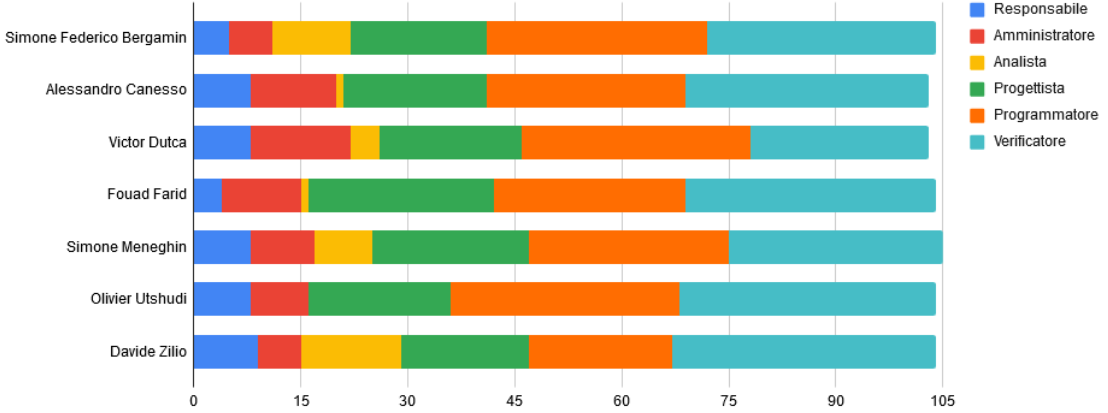
\includegraphics[scale=0.50]{img/grafici/consuntivo_ore.png}
\caption{Istogramma del consuntivo delle ore totali per ruolo senza investimento}
\end{figure}

\subsubsection{Conclusioni}
Il bilancio totale orario del nostro progetto risulta negativo perché sono state
necessarie 4 ore di lavoro in più rispetto a quanto preventivato.
Come si può notare dai consuntivi di periodo, i nostri bilanci sono sempre
migliorati col tempo, questo è dovuto al fatto che l’inesperienza iniziale non
ci ha permesso di individuare correttamente le ore necessarie per ciascun
ruolo in ogni periodo. Siamo tuttavia riusciti a non discostarci troppo da
quanto preventivato grazie alle continue rilevazioni dell’andamento del nostro
lavoro e la successiva applicazione di misure atte a mitigare gli scostamenti
osservati. In particolare, è risultato essenziale cambiare la pianificazione del
periodo di progettazione di dettaglio e codifica a seguito degli scostamenti
nel periodo di progettazione architetturale.
In conclusione possiamo quindi ritenerci soddisfatti perché con l’avanzare del tempo e l’incremento della nostra esperienza, siamo riusciti a migliorare la gestione delle risorse, intervenendo adeguatamente con le dovute accortezze.

\subsubsection{Preventivo a finire}
Il preventivo a finire, e quindi il bilancio totale economico, risulta positivo perché abbiamo speso meno di quanto pianificato (-10€). Anche nella gestione delle risorse economiche è risultata fondamentale l’attività di verifica continua che ci ha permesso di intervenire tempestivamente e di conseguenza adeguatamente, per non eccedere i costi presentati in sede di Revisione dei Requisiti. 
L’aggiornamento della pianificazione del periodo di progettazione di dettaglio
si è rilevato fondamentale a tale scopo.